\documentclass[a4paper,10pt]{report}

\usepackage[utf8]{inputenc}
\usepackage{amsmath}
\usepackage{amssymb}
\usepackage{amsfonts}
\usepackage{bm}
\usepackage{tikz}
\usepackage{pgfplots}
\usepackage{algorithm}
\usepackage{listings}
\usepackage[noend]{algpseudocode}
\usepackage[english,russian]{babel}


\title{Течение несжимаемой жидкости}
\author{Захаров ПЕ}

\begin{document}

\maketitle

\begin{abstract}
...
\end{abstract}



\chapter{Стационарное течение несжимаемой жидкости}

\section*{Введение}
Рассматривается численное моделирование стационарного течения несжимаемой жидкости. 

\section{Математические модели описания течений несжимаемой жидкости}

\subsection{Стационарное уравнение Навье-Стокса}

Течение жидкости описывается системой уравнений состоящей из уравнения для момента импульса и уравнения неразрывности. Для описания стационарного течения несжимаемой жидкости используются следующие уравнения в области $\Omega$
\begin{equation}
  \rho \,\mathcal{C}(\bm{u})
- \nabla \cdot \sigma(\bm{u}, p)
= \rho \bm{f},
\label{eq:navier-stokes}
\end{equation}
\begin{equation}
\nabla \cdot \bm{u} = 0,
\label{eq:incompressibility}
\end{equation}
где $\rho$ --- плотность, $\bm{u}(\bm{x})$ --- скорость жидкости, $\mathcal{C}(\bm{u})$ --- конвекция скорости, $\nabla$ --- оператор набла, $\cdot$ --- скалярное произведение, $\sigma(\bm{u}, p)=2 \mu \epsilon(\bm{u}) - p I$ --- тензор напряжения, $\mu$ --- вязкость, $\epsilon(\bm{u}) = \frac{1}{2}\left(\nabla \bm{u} + \nabla \bm{u}^T \right)$ --- тензор скорости деформации, $p$ --- давление, $I$ --- единичный оператор, $\bm{f}(\bm{x})$ --- объемные силы.

\subsection{Формы конвективной части}

Конвективную часть уравнения $\mathcal{C}(\bm{u})$ можно записывать в четырех различных формах, которые идентичны для непрерывных дифференциальных операторов, но различаются для дискретных операторов:
\begin{itemize}
\item $\nabla \cdot \left(\bm{u} \otimes \bm{u} \right)$ --- дивергентная форма;
\item $\bm{u} \cdot \nabla \bm{u}$ --- адвективная форма;
\item $\frac{1}{2}\left(\nabla \cdot \left(\bm{u} \otimes \bm{u} \right) + \bm{u} \cdot \nabla \bm{u} \right)$ --- кососимметричная форма;
\item $\left( \nabla \times \bm{u} \right) \times \bm{u} + \frac{1}{2} \nabla \left(\bm{u} \cdot \bm{u} \right) $ --- ротационная форма (rotation form);
\end{itemize}
где $\otimes$ --- тензорное произведение, $\times$ --- векторное произведение для трехмерной области, а для двумерной области $\nabla \times \bm{u} := -\frac{\partial u_1}{\partial x_2} + \frac{\partial u_2}{\partial x_1}$ и $a \times \bm{u} := (-a u_2, a u_1)^T$ для скаляра $a$


\subsection{Граничные условия}
Для задач течения жидкости стандартными являются следующие граничные условия
\begin{itemize}
\item условие прилипания (noslip condition) $\bm{u}(\bm{x}, t) = (0, 0)$;
\item условие скольжения или симметрии (slip condition) $\bm{u} \cdot \bm{n} = 0$;
\item условие на входе $\bm{u}(\bm{x}) = \bm{u}_{in}(\bm{x})$;
\item условие на выходе $p(\bm{x}) = p_{out}(\bm{x})$, $\nabla \bm{u} \cdot \bm{n} = 0$;
\item периодические граничные условия $\bm{u}(\bm{x}) = \bm{u}(\bm{x} + \bm{x}_{period})$;
\end{itemize}
где $\bm{n}$ --- внешняя нормаль границы. В некоторых задачах граничное условие для давления может не задаваться и тогда используется ограничение
\[
\int_\Omega p \; {\rm d}\bm{x} = 0,
\]
которое дает единственное решение для давления.

\section{Вычислительный алгоритм}

\subsection{Конечно-элементная аппроксимация}

Для задачи без ограничения для давления используется стандартная вариационная задача.
Для описания вариацонной формулировки уравнений умножаем на тестовые функции, итегрируем по области и понижаем порядок производных. Вариационная задача заключается в нахождении функций $\bm{u} \in V, p \in Q$, которые удовлетворяют
\begin{equation}
\begin{gathered}
F = \int_\Omega \rho \,\mathcal{C}(\bm{u}) \cdot \bm{v} \;{\rm d}\bm{x} 
 + \int_\Omega \sigma(\bm{u}, p) \cdot \epsilon(\bm{v}) \;{\rm d}\bm{x} \\
 - \int_\Gamma ... \\
 - \int_\Omega \rho \bm{f} \cdot \bm{v} \;{\rm d}\bm{x} 
 + \nabla \cdot \bm{u} q \;{\rm d}\bm{x} = 0,
\end{gathered}
\label{eq:nonlinear-form}
\end{equation}
где $\bm{u} \in V, p \in Q, \bm{v} \in \widehat{V}, q \in \widehat{Q}$.

Для аппроксимации скорости используется кусочно-квадратичные функции, а для давления --- кусочно-линейные функции, данная комбинация элементов известна как элементы Тэйлор-Худа.

\subsection{Численное решение дискретной задачи}

Рассмотрим стационарную задачу в единичном квадрате $\Omega=(0,1)^2$ с точным решением
\begin{equation}
\begin{gathered}
\bm{u}_e = \left(80 e^{x_1}(x_1 - 1)^2 x_1^2 x_2 (x_2 -  1) (2 x_2 - 1),\right.\\
\left. -40 e^{x_1} (x_1 - 1) x_1 (x_1 (3 + x_1) - 2) (x_2-1)^2 x_2^2\right), \\
p_e = 10 (-424 + 156 e + (x_2^2-x_2) (-456 + e^x_1) (456 + x_1^2) (228 - 5 (x_2^2 - x_2)) \\
+ 2 x_1 (-228 + (x_2^2 - x_2)) + 2 x_1^3 (-36 + x_2^2 - x_2)) + x_1^4 (12 + (x_2^2 - x_2))))).
\end{gathered}
\label{eq:shifted-vortex}
\end{equation}
Возьмем следующие параметры модели
\[
\rho = 1, \quad \mu = 0.01, \quad \bm{f} = \rho \,\mathcal{C}(\bm{u}_e) - \nabla \cdot \epsilon(\bm{u}_e, p_e).
\]
На рис. \ref{fig:shifted-vortex-u}, \ref{fig:shifted-vortex-p} показаны точные решения задачи.
%\begin{figure}[h]
%\centering
%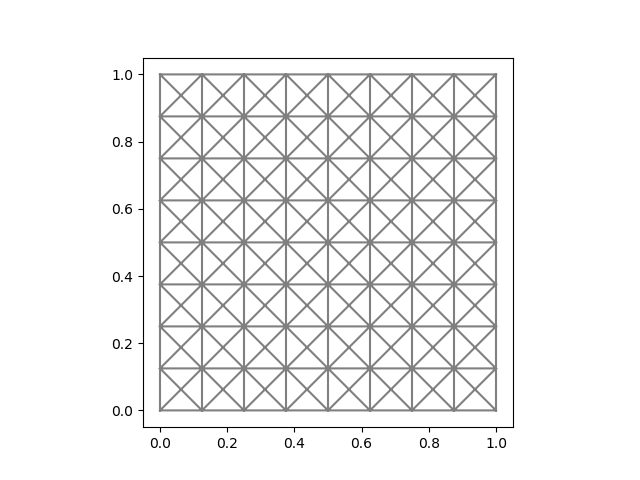
\includegraphics[width=1.0\linewidth]{shifted-vortex/mesh.png}
%\label{fig:mesh8}
%\caption{Вычислительная сетка $8 \times 8$}
%\end{figure}

\begin{figure}
\centering
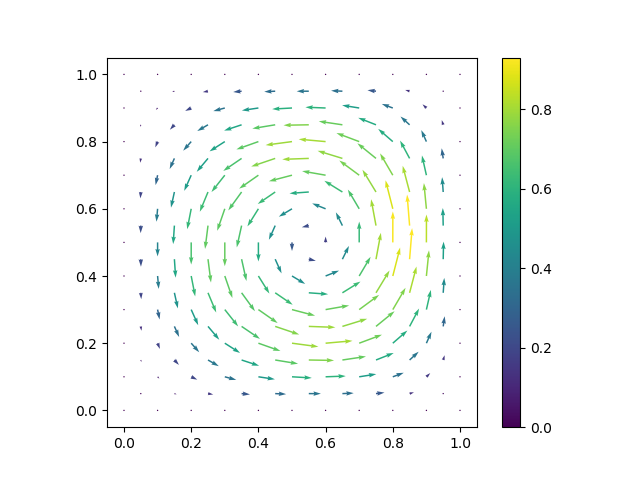
\includegraphics[width=0.49\linewidth]{shifted-vortex/u.png}
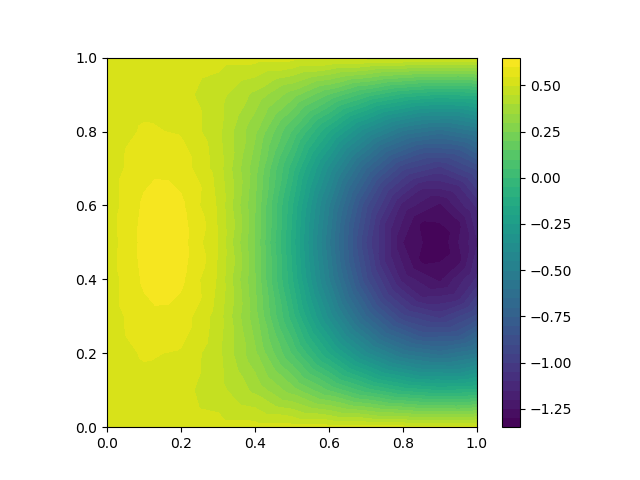
\includegraphics[width=0.49\linewidth]{shifted-vortex/p.png}
\label{fig:shifted-vortex}
\caption{Поле скорости и распределение давления}
\end{figure}

\section{Программная реализация}
...

\subsection{Общее описание}
...

\subsection{Структура ПО}
...

\subsection{Ключевые элементы (описание классов)}
...

\subsection{Листинг программы}
...

\section{Тестирование ПО}
...

\subsection{Тестовые задачи (для демонстрации сходимости в зависимости от вычислительных параметров, ...)}
...

\subsection{Сходимость аппроксимации по пространству}

Для исследования численного решения от размера вычислительной сетки рассматриваем последовательность сеток: $8\times8$, $16\times16$, $32\times32$, $64\times64$, $128\times128$. Сравниваются различные нормы погрешности скорости и давления: 
\[
\left\Vert \bm{u} - \bm{u}_e \right\Vert_{L^2}, \quad
\left\Vert \bm{u} - \bm{u}_e \right\Vert_{L^\infty}, \quad
\left\Vert \bm{u} - \bm{u}_e \right\Vert_{H^{div}_0},
\]
\[
\left\Vert p - p_e \right\Vert_{L^2}, \quad
\left\Vert p - p_e \right\Vert_{L^\infty}, \quad
\left\Vert p - p_e \right\Vert_{H^1_0}.
\]

\begin{figure}[h]
\centering
\begin{tikzpicture}[scale=1]
\begin{axis}[
	xmode=log,
	ymode=log,
    ylabel={$\varepsilon$},
    xlabel=$N$,
    grid=major,
    legend pos=north east]
    \addplot[mark=*,solid] table[y=eul2]{shifted-vortex/meshes.txt};
    \addplot[mark=*,dashed] table[y=eumax]{shifted-vortex/meshes.txt};
    \addplot[mark=*,dotted] table[y=euhd0]{shifted-vortex/meshes.txt};
    \addlegendentry{$L^2$}
    \addlegendentry{$L^\infty$}
    \addlegendentry{$H^{div}_0$}
\end{axis}
\end{tikzpicture}
\caption{Зависимость нормы погрешности скорости от размера сетки $N \times N$}
\label{fig:shifted-vortex-meshes-u}
\end{figure}
\begin{figure}[h]
\centering
\begin{tikzpicture}[scale=1]
\begin{axis}[
	xmode=log,
	ymode=log,
    ylabel={$\varepsilon$},
    xlabel=$N$,
    grid=major,
    legend pos=north east]
    \addplot[mark=*,solid] table[y=epl2]{shifted-vortex/meshes.txt};
    \addplot[mark=*,dashed] table[y=epmax]{shifted-vortex/meshes.txt};
    \addplot[mark=*,dotted] table[y=eph10]{shifted-vortex/meshes.txt};
    \addlegendentry{$L^2$}
    \addlegendentry{$L^\infty$}
    \addlegendentry{$H^1_0$}
\end{axis}
\end{tikzpicture}
\caption{Зависимость нормы погрешности давления от размера сетки $N \times N$}
\label{fig:shifted-vortex-meshes-p}
\end{figure}

\subsection{Прямые линейные решатели}

Из сравнения прямых решателей (см. рис. \ref{fig:direct-solvers}) наилучшее время показал MUMPS, который имеет параллельное решение системы. На рис. \ref{fig:mumps-parallel} приводится сравнение времени параллельного решения решателем MUMPS для вычислительных сеток $128\times128$ и $256\times256$.

\begin{figure}[h]
\centering
\begin{tikzpicture}[scale=1]
\begin{axis}[
	xmode=log,
	ymode=log,
    ylabel={$t, s$},
    xlabel=$N$,
    grid=major,
    legend pos=north west]
    \addplot[mark=*,solid] table[y=mumps]{shifted-vortex/direct-solvers.txt};
    \addplot[mark=*,dashed] table[y=petsc]{shifted-vortex/direct-solvers.txt};
    \addplot[mark=*,dashdotted] table[y=umfpack]{shifted-vortex/direct-solvers.txt};
    \addplot[mark=*,dotted] table[y=superlu]{shifted-vortex/direct-solvers.txt};
    \addlegendentry{MUMPS}
    \addlegendentry{PETSc}
    \addlegendentry{UMFPack}
    \addlegendentry{SuperLU}
\end{axis}
\end{tikzpicture}
\caption{Время решения прямых решателей от размера сетки $N \times N$}
\label{fig:direct-solvers}
\end{figure}
\begin{figure}[h]
\centering
\begin{tikzpicture}[scale=1]
\begin{axis}[
	xmode=log,
	ymode=log,
    ylabel={$t, s$},
    xlabel=$P$,
    grid=major,
    legend pos=north east]
    \addplot[mark=*,solid] table[y=N128]{shifted-vortex/mumps-parallel.txt};
    \addplot[mark=*,dashed] table[y=N256]{shifted-vortex/mumps-parallel.txt};
    \addplot[mark=*,dotted] table[y=N512]{shifted-vortex/mumps-parallel.txt};
    \addlegendentry{$N=128$}
    \addlegendentry{$N=256$}
    \addlegendentry{$N=512$}
\end{axis}
\end{tikzpicture}
\caption{Время решения решателя MUMPS от количества процессов $P$}
\label{fig:mumps-parallel}
\end{figure}

\subsection{Итерационные линейные решатели}
...

\subsection{Преобуславливатели линейных решателей}
...

\subsection{Результаты по параллелизации}
...


\section{Верификация ПО}
...

\subsection{Матрица верификации (общее описание набор задач)}
...

\subsection{Задача 1}
...


%\bibliographystyle{unsrt}
%\bibliography{literature}

\end{document}
